\section{Histogramme}

\subsection{Überlegungen}
Jetzt wo ich die Kreiserkennung implementiert habe, ist es mir möglich Münzen im Bild zu erkennen. Der nächste Schritt wäre es nun, die Münzen zu klassifizieren und zu unterscheiden. Doch wie klassifiziert man in openCV Bilder? Meine Idee war es, die Bilder als Histogramme zu speichern und zu vergleichen. Ein Histogramm ist eine graphische Darstellung der Häufigkeitsverteilung von Werten. In meinem Fall würde ich die Farbwerte der Münzen in einem Histogramm speichern und diese dann vergleichen.

\subsection{Die Vorlagen}
Damit ich die Münzen anhand ihrer Bildinformastionen klassifizieren kann, benötige ich zuerst Vorlagen, mit denen ich die Münzen vergleichen kann. Ich habe also Bilder von den Münzen gemacht und diese als Vorlagen gespeichert. Diese Vorlagenbilder sind die Referenzbilder, anhand derer ich die Münzen im Kamerabild auf Ähnlichkeit überprüfen möchte.

Hier hat sich vorallem die spiegelnde Oberfläche der Münzen als Problem herausgestellt. Ich musste viel mit dem Lichteinfallswinkel und der Beleuchtung spielen, um von jeder Münze ein gutes Bild zu bekommen. Auch der Abnutzungsgrad hat das Erstellen der Vorlagen erschwert. So musste ich vorallem bei den 50-20-10 Cent Münzen und bei den 5-2-1 Cent Münzen darauf achten, dass die Münzen stets eine ähnliche Optik ausweisen. Andernfalls könnte es passieren, dass die Spiegelung oder die Abnutzung als Unterschied interpretiert wird und nicht mehr die Ziffern auf den Münzen.

Meine Vorlagen sehen wie folgt aus:

\begin{figure}[ht]
    \centering
    \begin{subfigure}{0.23\textwidth}
        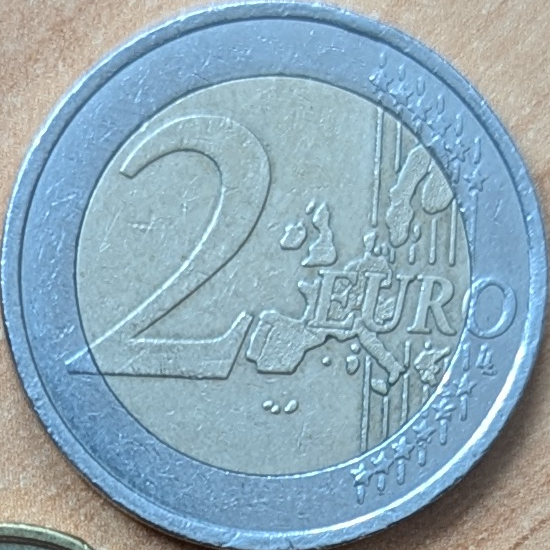
\includegraphics[width=\linewidth]{../CoinFinder/templates_2/Euro2.png}
    \end{subfigure}
    \begin{subfigure}{0.23\textwidth}
        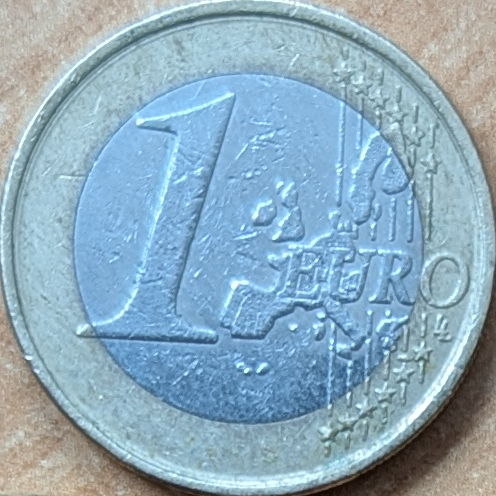
\includegraphics[width=\linewidth]{../CoinFinder/templates_2/Euro1.png}
    \end{subfigure}
    \begin{subfigure}{0.23\textwidth}
        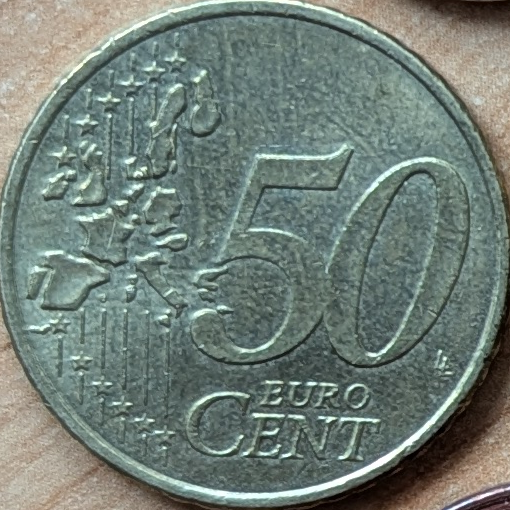
\includegraphics[width=\linewidth]{../CoinFinder/templates_2/Cent50.png}
    \end{subfigure}
    \begin{subfigure}{0.23\textwidth}
        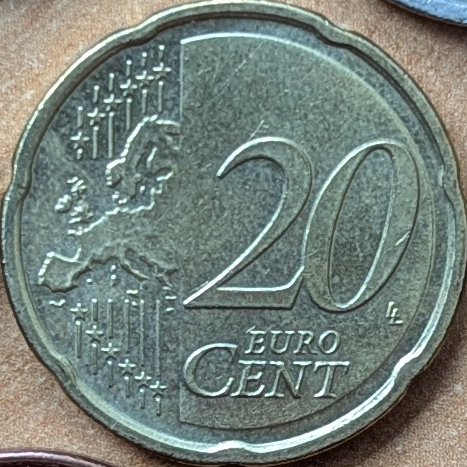
\includegraphics[width=\linewidth]{../CoinFinder/templates_2/Cent20.png}
    \end{subfigure}

    \begin{subfigure}{0.23\textwidth}
        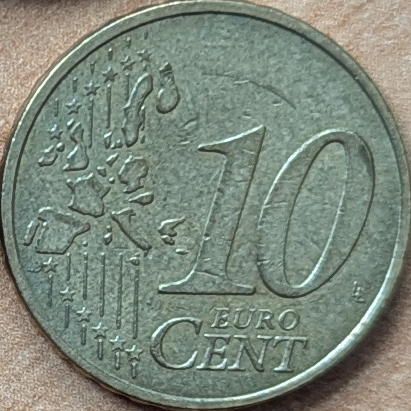
\includegraphics[width=\linewidth]{../CoinFinder/templates_2/Cent10.png}
    \end{subfigure}
    \begin{subfigure}{0.23\textwidth}
        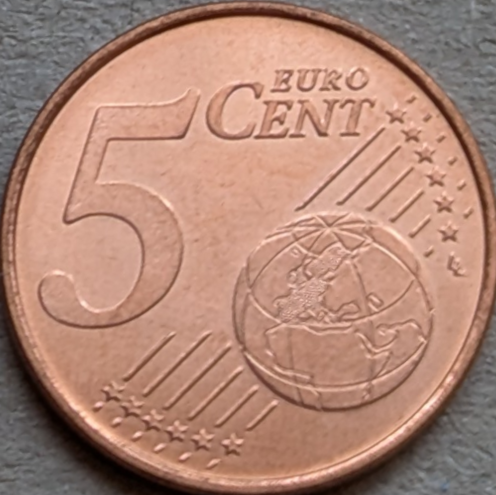
\includegraphics[width=\linewidth]{../CoinFinder/templates_2/Cent5.png}
    \end{subfigure}
    \begin{subfigure}{0.23\textwidth}
        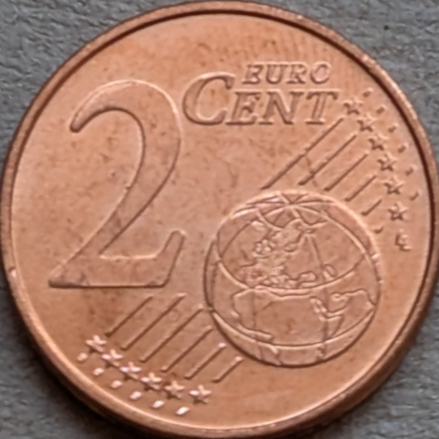
\includegraphics[width=\linewidth]{../CoinFinder/templates_2/Cent2.png}
    \end{subfigure}
    \begin{subfigure}{0.23\textwidth}
        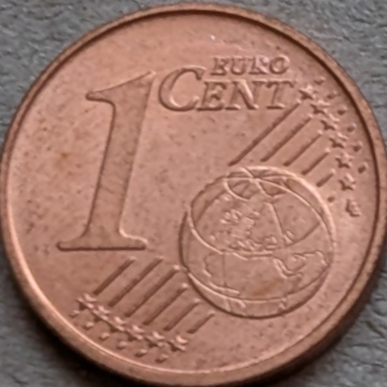
\includegraphics[width=\linewidth]{../CoinFinder/templates_2/Cent1.png}
    \end{subfigure}
\end{figure}

\subsection{Erstellung der Histogramme}
Als nächstes habe ich mich mit der Erstellung der Histogramme beschäftigt. Grundlegend kann man in openCV ein Histogramm mit der folgenden Funktion erstellen:

\begin{lstlisting}[language=JavaScript]
cv.calcHist(images, channels, mask, hist, histSize, ranges);
\end{lstlisting}

\begin{itemize}
    \item \textbf{images} - Die Bilder, die berücksichtigt werden sollen. Die Funktion erwartet ein Parameter vom Typ MatVector, also ein Array von Mat-Objekten. In meinem Fall muss ich für jedes Histogramm ein MatVector-Objekt erstellen, das nur das eine Matrix enthält.
    \item \textbf{channels} - Die Farbkanäle, die berücksichtigt werden sollen.
    \item \textbf{mask} - Eine Maske, die angibt, welche Pixel berücksichtigt werden sollen. In meinem Fall benutze ich eine kreisrunde Maske mit dem Radius der Hälfte des Bildes. So ist bei einer Münze die das gesamte Bild vollständig einnimmt sichergestellt, dass die Ränder des Bildes nicht in die Berechnung des Histogramms einfließen.
    \item \textbf{hist} - Das Histogramm, das erstellt wird. Die Funktion erwartet ein Mat-Objekt, in das das Histogramm geschrieben wird.
    \item \textbf{histSize} - Die Anzahl der Bins, also die Anzahl der Werte, die das Histogramm haben soll. Ein Bin ist ein Bereich von Werten, die zusammengefasst werden. In meinem Fall habe ich 256 Bins, da die Farbwerte von 0-255 gehen.
    \item \textbf{ranges} - Der Bereich der Werte, die das Histogramm haben soll. In meinem Fall gehen die Farbwerte von 0-255.
\end{itemize}

Bevor ich nun mit der Erstellung der Histogramme beginne, brauche ich zunächst eine Möglichkeit um sowohl die Vorlagen als auch die künftigen Hisogramme zu speichern und ihnen eine Münze zuzuordnen. Dafür habe ich ein global verfügbares Objekt \textit{COINS} erstellt, welches die Münzen als Schlüssel enthält und als Wert ein Objekt mit den Eigenschaften \textit{diameter} und \textit{value} hat. Weitere Eigenschaften können dann zur Laufzeit den einzelnen Münzen hinzugefügt werden.

\begin{lstlisting}[style=JavaScript]
let COINS = {
    Euro2 : {
        diameter: 25.75,
        value: 2
    },
    Euro1 : {
        diameter: 23.25,
        value: 1
    },
    Cent50 : {
        diameter: 24.25,
        value: 0.5
    },
    Cent20 : {
        diameter: 22.25,
        value: 0.2
    },
    Cent10 : {
        diameter: 19.75,
        value: 0.1
    },
    Cent5 : {
        diameter: 21.25,
        value: 0.05
    },
    Cent2 : {
        diameter: 18.75,
        value: 0.02
    },
    Cent1 : {
        diameter: 16.25,
        value: 0.01
    }
}    
\end{lstlisting}

Diese Datenstruktur kann ich nun verwenden, um die Histogramme zu speichern und ihnen eine Münze zuzuordnen. In der folgenden Methode iteriere ich über jede Münze und lese das Vorlagenbild ein. Anschließend erstelle ich aus diesem ein Hisogramm und speichere es in der globalen Datenstruktur. Die Methode sieht so aus:

\begin{lstlisting}[style=JavaScript]
function InitHists(){

    Object.entries(COINS).forEach(([key, value]) => {
        //is in the template folder a picture with the same name as the key?
        let img = new Image();

        img.onload = () => {
            console.log("loaded: " + key);

            let src = cv.imread(img); //convert image to matrix
            let histSize = [256];
            let range = [0, 255];

            let channels = new cv.MatVector();
            cv.split(src, channels);

            //histogramms for each channel
            let redHist = new cv.Mat();
            let greenHist = new cv.Mat();
            let blueHist = new cv.Mat();

            //create mask for the circle
            let mask = cv.Mat.zeros(src.rows, src.cols, cv.CV_8UC1); //create a black image
            let center = new cv.Point(src.cols/2, src.rows/2);
            let radius = src.cols/2;
            cv.circle(mask, center, radius, [255, 255, 255, 255], -1); //draw a white circle in the middle of the image

            //calculate histogramm for each channel
            let matVec = new cv.MatVector();
            matVec.push_back(src);
            cv.calcHist(matVec, [0], mask, redHist, histSize, range, false);
            cv.calcHist(matVec, [1], mask, greenHist, histSize, range, false);
            cv.calcHist(matVec, [2], mask, blueHist, histSize, range, false);

            //normalize histograms
            cv.normalize(redHist, redHist, 0, 255, cv.NORM_MINMAX);
            cv.normalize(greenHist, greenHist, 0, 255, cv.NORM_MINMAX);
            cv.normalize(blueHist, blueHist, 0, 255, cv.NORM_MINMAX);

            COINS[key].hist = [redHist, greenHist, blueHist];

            //free memory
            src.delete();
            channels.delete();
            mask.delete();
            matVec.delete();
        }

        img.onerror = () => {
            console.log("error: " + key);
        }

        img.src = path + key + ".png";

    });
}
\end{lstlisting}

Wie man sehen kann erstelle ich testweise erstmal für jeden Farbkanal ein eigenes Histogramm, um später herauszufinden welcher Kanal am besten geeignet ist. Zusätzlich normalisiere ich alle Hisogramme, um "Lücken" in den Histogrammen zu vermeiden. Dafür kann die Funktion \textit{cv.normalize} verwendet werden, welche in meinem Beispiel die Histogramme direkt im Speicher überschreibt.

\subsection{Vergleich der Histogramme}
Nun brauchen einen Weg jene vorgespeicherten Histogramme mit den Histogrammen der Kamerabilder zu vergleichen. Dafür habe ich eine Methode \textit{CompareHists} erstellt, die die Histogramme vergleicht und die Münze mit dem geringsten Unterschied zurückgibt. Die Methode sieht so aus:

\subsection{Erste Ergebnisse}
Es hat sich gezeigt, dass der Vergleich von Histogrammen prinzipiell funktioniert. Allerdings ist die Genauigkeit noch nicht zufriedenstellend. Münzen können zwar grob in die richtige Kategorie eingeordnet werden (sprich 1-2-5 Cent Münzen und 10-20-50 Cent Münzen), jedoch ist die Unterscheidung innerhalb dieser Kategorien nicht funktional.

Es scheint, dass die Ziffern der Euromünzen nicht ausreichend in den Histogrammen repräsentiert sind. Die Histogramme der Münzen sind sich zu ähnlich, sodass die Unterschiede nicht ausreichend hervorgehoben werden. Ich muss mich also nach weiteren Mölichkeiten umsehen, um Münzen zuverlässig und eindeutig zu klassifizieren.